\chapter{NetXPTO Implementation}
\label{chapter4}


This chapter consists in an overview of the created platform, in which the developed heuristic algorithms were implemented. The starting point was the NetXPTO-Netplanner open source simulator, which is a real-time simulator that allows the creation of generic systems comprised of a set of blocks that interact with each other through signals. The NetXPTO-NetPlanner has been developed by several people using git as a version control system and its repository is located in the GitHub site https://github.com/netxpto/NetPlanner. This chapter is organized in six subsections where a general description is given on how the platform was implemented and on how it operates in practical terms. In section \ref{ips} is presented an explanation on which are the accepted entry parameters of the system and how they can be provided, on section \ref{lf} is addressed the functionality of the log file and how to access it and on section \ref{tss} the type of existent signals and which information they carry and share between blocks. On section \ref{fr} a generic description is given on how to interpret the final report generated by the system after running each simulation and finally more generic information about each block input parameters/signals, state variables and output signals is present in section \ref{practical}.  


\definecolor{mygreen}{rgb}{0,0.6,0}
\definecolor{mygray}{rgb}{0.5,0.5,0.5}
\definecolor{mymauve}{rgb}{0.58,0,0.82}

\lstset{ %
	backgroundcolor=\color{white},   % choose the background color; you must add \usepackage{color} or \usepackage{xcolor}; should come as last argument
	basicstyle=\footnotesize,        % the size of the fonts that are used for the code
	breakatwhitespace=false,         % sets if automatic breaks should only happen at whitespace
	breaklines=true,                 % sets automatic line breaking
	captionpos=b,                    % sets the caption-position to bottom
	commentstyle=\color{mygreen},    % comment style
	deletekeywords={...},            % if you want to delete keywords from the given language
	escapeinside={\%*}{*)},          % if you want to add LaTeX within your code
	extendedchars=true,              % lets you use non-ASCII characters; for 8-bits encodings only, does not work with UTF-8
	frame=single,	                   % adds a frame around the code
	keepspaces=true,                 % keeps spaces in text, useful for keeping indentation of code (possibly needs columns=flexible)
	keywordstyle=\color{blue},       % keyword style
	language=Octave,                 % the language of the code
	morekeywords={*,...},            % if you want to add more keywords to the set
	numbers=left,                    % where to put the line-numbers; possible values are (none, left, right)
	numbersep=5pt,                   % how far the line-numbers are from the code
	numberstyle=\tiny\color{mygray}, % the style that is used for the line-numbers
	rulecolor=\color{black},         % if not set, the frame-color may be changed on line-breaks within not-black text (e.g. comments (green here))
	showspaces=false,                % show spaces everywhere adding particular underscores; it overrides 'showstringspaces'
	showstringspaces=false,          % underline spaces within strings only
	showtabs=false,                  % show tabs within strings adding particular underscores
	stepnumber=2,                    % the step between two line-numbers. If it's 1, each line will be numbered
	stringstyle=\color{mymauve},     % string literal style
	tabsize=2,	                   % sets default tabsize to 2 spaces
	title=\lstname                   % show the filename of files included with \lstinputlisting; also try caption instead of title
}
\section{Input Parameters System}
\label{ips}

The execution of a simulation is mainly based in three files. Initially, there is an \textbf{input\_parameters\_values.txt} file, which contains all the entry variables that the system needs in order to run correctly, however, if any of the variables is missing or incorrectly declared then the default value defined for that variable is considered, they can be consulted below in table \ref{system_input}. There is also an executable file named \textbf{transparent.exe} generated after compiling the project, which  will load the entry variables values from the previously mentioned text file, run the simulation and later on print the final results in an other text file, \textbf{FinalReport.txt}.\\ \\

The purpose of this section is to describe the \gls{ips} which enables the reading of input parameters values from any text file.

\subsection{Entry variables}
The system input parameters are described below in table \ref{system_input} and their respective default values are given.  
\begin{table}[H]
	\centering
	\scalebox{0.65}{
\begin{tabular}{|c|c|c|}
\hline
\textbf{Parameter} & \textbf{Default value} & \textbf{Description} \\ \hline
numberOfNodes & 0 & \begin{tabular}[c]{@{}c@{}}Number of existing nodes\\ in the network.\end{tabular} \\ \hline
odu0 & {[}0{]} & \begin{tabular}[c]{@{}c@{}}N by N matrix containing\\ ODU0 demands.\end{tabular} \\ \hline
odu1 & {[}0{]} & \begin{tabular}[c]{@{}c@{}}N by N matrix containing\\ ODU1 demands.\end{tabular} \\ \hline
odu2 & {[}0{]} & \begin{tabular}[c]{@{}c@{}}N by N matrix containing\\ ODU2 demands.\end{tabular} \\ \hline
odu3 & {[}0{]} & \begin{tabular}[c]{@{}c@{}}N by N matrix containing\\ ODU3 demands.\end{tabular} \\ \hline
odu4 & {[}0{]} & \begin{tabular}[c]{@{}c@{}}N by N matrix containing\\ ODU4 demands.\end{tabular} \\ \hline
orderingRule & descendingOrder & \begin{tabular}[c]{@{}c@{}}descendingOrder (ODU4...0)\\ ascendingOrder (ODU0...4)\end{tabular} \\ \hline
transportMode & transparent & \begin{tabular}[c]{@{}c@{}} This dissertation focus only on\\ the transparent mode approach\end{tabular} \\ \hline
physicalTopologyAdjacencyMatrix & {[}0{]} & \begin{tabular}[c]{@{}c@{}}N by N matrix containing\\ existent physical connections\\between nodes.\end{tabular} \\ \hline
numberOfTSPerLink & 1 & \begin{tabular}[c]{@{}c@{}}Number of transmission\\ systems existing\\  in each physical link.\end{tabular} \\ \hline
numberOfOpticalChannelsPerLink & 100 & \begin{tabular}[c]{@{}c@{}}Number of optical channels\\ per physical link.\end{tabular} \\ \hline
initialWavelenght & 1550 & \begin{tabular}[c]{@{}c@{}}Initial value of the wavelength\\ used expressed in nanometers.\end{tabular} \\ \hline
wavelengthSpacing & 0.8 & \begin{tabular}[c]{@{}c@{}}Interval between used\\ wavelengths. (nm)\end{tabular} \\ \hline
opticalChannelCapacity & 80 & \begin{tabular}[c]{@{}c@{}}Physical capacity of each \\ optical channel expressed in\\ number of ODU0 demands.\end{tabular} \\ \hline
distancesBetweenNodes & [0] & \begin{tabular}[c]{@{}c@{}}N by N matrix containing\\ distances between node sites.\end{tabular} \\ \hline
routingCriterionLogicalTopology & Hops & Shortest path type. \\ \hline
routingCriterionPhysicalTopology & Hops & Shortest path type. \\ \hline
blockingCriterionLogicalTopology & 1 & \begin{tabular}[c]{@{}c@{}}Number of shortest logical\\ paths generated by the routing\\ algorithm.\end{tabular} \\ \hline
blockingCriterionPhysicalTopology & 3 & \begin{tabular}[c]{@{}c@{}}Number of shortest physical\\ paths generated by the routing\\ algorithm.\end{tabular} \\ \hline
\end{tabular}}
	\caption{System input parameters.}
	\label{system_input}
\end{table}

\subsection{Format of the Input File}
The input file to run this simulator must respect the following properties:
\begin{enumerate}
	\item Input parameter values can be changed by adding a line in the following format:
\textbf{paramName=newValue}, where paramName represents the name of the input parameter and
newValue the value to be assigned.
    \item In the case of an input paramenter of the matrix type, ODU traffic matrices and/or physical and logical topologies, newValue will assume the value of existing elements per line or column and the matrix value must be specified below this line.
    \item If an input parameters is assigned the wrong type of value, method
readSystemInputParameters() will throw an exception.
    \item In the case and input parameter is not assigned with a specific value it will assume the default value.
    \item The IPS supports comments in the form of the characters //. The comments will only
be recognized if placed at the beginning of a line.
\end{enumerate}

An example of the \textbf{input\_parameters\_values.txt} used to load values into the simulator, for a network with 6 nodes, is shown below. \\ \\

\lstinputlisting[language=C++, caption=input\_parameters\_values.cpp code]{fig/logos/input_parameters_values.cpp}

\subsection{Loading Input Parameters From A File}
 Execute the following command in the Command Line:\\

\textbf{transparent.exe<input\_file\_path><output\_directory>}\\

where transparent.exe is the name of the executable generated after compiling the project, <input\_file\_path> is the path to the file containing the new input parameters; <output\_directory> is the directory where the output signals will be written into. The final report file, \textbf{FinalReport.txt}, will be written the directory of the project itself.

\section{Log File}
\label{lf}
The Log File allows for a detailed analysis of a simulation. It will output a file named \textbf{log.txt} containing the timestamp of when a block is initialized, the number of samples in the buffer ready to be processed for each input signal, the signal buffer space for each output signal and the amount of time in seconds that took to run each block. This will occur in each and every cycle until the system terminates the simulation. 

\section{Type signals structure}
\label{tss}

\subsection{Logical Topology}

A Logical Topology type signal contains numerous data structures that comprise the logical layer of the network. Below those structures are represented.

\subsubsection{Logical Topology Adjacency Matrix}

 The possible logical connections between a pair of nodes is demonstrated below on table \ref{physical_topology1}, where 1 and 0 represent the existence or not of a connection, respectively. 

\begin{table}[H]
	\centering	
	\begin{tabular}{|c|c|c|ccc|c|}
		\hline
		\textbf{Nodes} & 1 & 2 & \multicolumn{3}{c|}{...} & N \\ \hline
		1 & \textbf{0} & 0/1 & \multicolumn{3}{c|}{...} & 0/1 \\ \hline
		2 & 0/1 & \textbf{0} & \multicolumn{3}{c|}{...} & 0/1 \\ \hline
		\textbf{.} & \textbf{.} & \textbf{.} & \textbf{.} &  &  & \textbf{.} \\
		\textbf{.} & \textbf{.} & \textbf{.} &  & \textbf{.} &  & \textbf{.} \\
		\textbf{.} & \textbf{.} & \textbf{.} &  &  & \textbf{.} & \textbf{.} \\ \hline
		N & 0/1 & 0/1 & \multicolumn{3}{c|}{...} & \textbf{0} \\ \hline
	\end{tabular}
	\caption{Allowed logical topology for a network of N nodes.}
	\label{physical_topology1}
\end{table}

 Here, value N represents the number of nodes present in the network. During this dissertation, the focus was on the transparent mode, where each node connects to all others creating direct logical links between all nodes of the network. The next considered variables are distributed in an hierarchical way as a path consists in one or more lightpaths which in its own turn are formed by one or more optical channels from distinct physical links.

\subsubsection{Path}

\begin{table}[H]
	\centering
	\scalebox{0.8}{
	\begin{tabular}{|c|c|c|c|c|c|}
		\hline
		Path Index & Source Node & Destination Node & \begin{tabular}[c]{@{}c@{}}Capacity\\ (ODU0s)\end{tabular} & Number of Lightpaths& Lightpaths Index\\ \hline
		Integer (>=0) & 1...N & 1...N & Integer (>0) & Integer (>=0) & {[}lp\_1, lp\_2, ...{]} \\ \hline
	\end{tabular}}
	\caption{Structure of a "Path" variable.}
	\label{path}
\end{table}

It represents a unique route identified by an index, containing one or more lightpaths and assigned to specific connection request, where for example lp\_1 and lp\_2 represent the lightpaths with index number 1 and 2, respectively. The capacity available of each path is given in terms of quantity of ODU0 demands.

\subsubsection{Lightpath}

\begin{table}[H]
	\centering
	\scalebox{0.8}{
\begin{tabular}{|c|c|c|c|c|c|}
	\hline
	Lightpath Index & Source Node & Destination Node & \begin{tabular}[c]{@{}c@{}}Capacity\\ (ODU0s)\end{tabular} & \begin{tabular}[c]{@{}c@{}}Number of\\ Optical Channels\end{tabular} & \begin{tabular}[c]{@{}c@{}}Optical Channels\\ Index\end{tabular} \\ \hline
	Integer (>=0) & 1...N & 1...N & Integer (>0) & Integer (>=0) & {[}och\_1, och\_2,...{]} \\ \hline
\end{tabular}}
	\caption{Structure of a "Lightpath" variable.}
	\label{lightPath}
\end{table}

It represents a set of one or more optical channels that transport information, from source to the destination node, while forcing data to remain in the optical domain without any \gls{o-e-o} conversion in between \cite{lightpath}. Each lightpath is identified by an unique index and its capacity is also expressed in quantities of ODU0 demands. The number and the indexes of the optical channels that comprise each lightpath are provided, where variables och\_1 and och\_2 represent the optical channels with index number 1 and 2, respectively.

\subsubsection{Optical Channel}

\begin{table}[H]
	\centering
	\scalebox{0.85}{
\begin{tabular}{|c|c|c|c|c|c|c|}
	\hline
	\begin{tabular}[c]{@{}c@{}}Optical Channel\\ Index\end{tabular} & Source Node & \begin{tabular}[c]{@{}c@{}}Destination\\ Node\end{tabular} & \begin{tabular}[c]{@{}c@{}}Capacity\\ (ODU0s)\end{tabular} &  \begin{tabular}[c]{@{}c@{}}Wavelenght\\ (nm)\end{tabular} & \begin{tabular}[c]{@{}c@{}}Number of\\ Demands\end{tabular} & \begin{tabular}[c]{@{}c@{}}Demands\\ Index\end{tabular} \\ \hline
	Integer (>=0) & 1...N & 1...N & Integer (>=0) & Real(>0) & Integer (>=0) & {[}d\_1, ...{]} \\ \hline
\end{tabular}}
	\caption{Structure of an "Optical Channel" variable.}
	\label{opticalChannels}
\end{table}

Each optical channel is identified by an unique index. The wavelength used in each channel is expressed in terms of nanometers (nm) and the number of demands carried through as well their index is recorded. Here d\_1 represents the demand with index number 1.

\subsection{Physical Topology}

 The allowed physical topology is defined by the duct and sites in the field \cite{TiagoEsteves}. It is assumed that each duct supports up to 2 unidirectional fiber links that together will behave like a bidirectional connection between a pair of nodes. Also each site supports up to 1 node. Below are represented the data structures that comprise signals of this type.

\subsubsection{Physical Topology Adjecency Matrix}

\begin{table}[H]
	\centering	
	\begin{tabular}{|c|c|c|ccc|c|}
		\hline
		\textbf{Nodes} & 1 & 2 & \multicolumn{3}{c|}{...} & N \\ \hline
		1 & \textbf{0} & 0/1 & \multicolumn{3}{c|}{...} & 0/1 \\ \hline
		2 & 0/1 & \textbf{0} & \multicolumn{3}{c|}{...} & 0/1 \\ \hline
		\textbf{.} & \textbf{.} & \textbf{.} & \textbf{.} &  &  & \textbf{.} \\
		\textbf{.} & \textbf{.} & \textbf{.} &  & \textbf{.} &  & \textbf{.} \\
		\textbf{.} & \textbf{.} & \textbf{.} &  &  & \textbf{.} & \textbf{.} \\ \hline
		N & 0/1 & 0/1 & \multicolumn{3}{c|}{...} & \textbf{0} \\ \hline
	\end{tabular}
	\caption{Allowed physical topology for a network of N nodes.}
	\label{physical_topology}
\end{table}

Here, the value 1 simply indicates the existence of a physical link between a pair of nodes and 0 symbolizes the absence of it.


\subsubsection{Link}

Based on the physical topology adjacency matrix variable another data structure is created for each of the existent physical links.

\begin{table}[H]
	\centering
	\scalebox{0.85}{
	\begin{tabular}{|c|c|c|c|c|c|c|}
		\hline
		\begin{tabular}[c]{@{}c@{}}Link Index\end{tabular} & Source Node & \begin{tabular}[c]{@{}c@{}}Destination\\ Node\end{tabular} & \begin{tabular}[c]{@{}c@{}}Number of\\ Wavelengths\end{tabular} & Wavelengths & \begin{tabular}[c]{@{}c@{}}Available\\ Wavelengths\end{tabular} & Amplifiers\\ \hline
		0...L-1 & 1...N & 1...N & OC & {[}w\_1, w\_2, ...{]} & {[}0/1 ... 0/1{]} & Integer (>=0) \\ \hline
	\end{tabular}}
	\caption{Structure of a "Link" variable.}
	\label{PhysicalGeneratorOut}
\end{table}

\vspace{11pt}
\noindent
where:
\begin{itemize}
\item{$OC$			$\rightarrow$	Number of existent optical channels in a link}
\item{$L$	$\rightarrow$	Number of unidirectional links in the network}
\item{$w\_1$	$\rightarrow$	Wavelength value with the index number 1 associated}
\end{itemize}

Once again, 1 and 0 indicates if the corresponding wavelength value is available or already being used, respectively. Other aspects as the quantity of wavelengths available per fiber, as well as its values, should also be discriminated. Regarding the capacity of each optical channel/wavelength, it can be expressed in different formats, for example, in terms of Gbit/s or in terms of the ODU0 demands, the lower unit of traffic considered. Finally, the number of needed amplifiers will depend of the length of the link and the assumed span value.

\subsection{Demand Request}

\begin{table}[H]
\centering
\scalebox{0.9}{
	\begin{tabular}{|c|c|c|c|l|}
		\hline
		\textbf{Demand Index} & \textbf{Source Node} & \textbf{Destination Node} &  \textbf{ODU Type} & \multicolumn{1}{c|}{\textbf{Survivability Method}}                                                 \\ \hline
		0...D-1       & 1...N       & 1...N            & 0...4    & \begin{tabular}[c]{@{}l@{}} none\\ protection\_1\_plus\_1\\ restoration\end{tabular} \\ \hline
	\end{tabular}}
	\caption{Constitution of a 'Demand Request' type signal.}
	\label{DemandRequest_variable}
\end{table}

A "Demand Request" type signal stands for a unique traffic request, where $D$ represents the total number of demand requests entering the network. It is possible to know the number of total unidirectional demands once we are dealing with static traffic and so all the traffic requests are known. In the situation where all requests for traffic are not known, the traffic is said to be dynamic. Regarding the survivability method, in this dissertation the work developed only considered the existence of none. 


\subsection{Path Request}

\begin{table}[H]
	\centering
	\scalebox{0.85}{
	\begin{tabular}{|c|c|c|c|c|c|}
		\hline
		Request Index & Demand Index & ODU Type & Source Node & Intermediate Nodes & Destination Node\\ \hline
		Integer (>=0) & 0...D-1& 0...4& 1...N      & 1...N             & 1...N          \\ \hline
	\end{tabular}}
	\caption{Constitution of a "Path Request" type signal.}
	\label{PathRequest}
\end{table}

A "Path Request" type signal is sent with an unique identifying index, from the logical topology manager block to the physical topology manager block asking for a path to be created between the source and destination nodes of a demand. In order establish that path, one or more lightpaths may be required, in the case there are intermediate nodes. In this specific case, transparent transport mode, only direct logical connections are taken into account, once, as previously mentioned, the information has to travel in the optical domain from source to destination, and so all paths created will be formed by only one direct lightpath. This means that in this specific scenario there will be no intermediate nodes, and when this happens the assumed value for this variable will be -1.

\subsection{Path Request Routed}

A "Path Request Routed" type signal contains the response from the physical topology manager block to a "Path Request" signal, indicating whether or not it is possible to establish a path requested for a demand. It is formed by the following data structures specified in tables \ref{pathInformation} and \ref{lpt}.

\subsubsection{Path Information}  
\begin{table}[H]
	\centering
	\begin{tabular}{|c|c|c|c|c|}
		\hline
		Request Index & Demand Index & ODU Type & Routed & Number of Lightpaths \\ \hline
		Integer (>=0) & D-1 &0...4 & True or False & \begin{tabular}[c]{@{}c@{}}Integer greater\\ or equal to 0\end{tabular} \\ \hline
	\end{tabular}
	\caption{Structure of a "Path Information" variable.}
	\label{pathInformation}
\end{table}

\subsubsection{Lightpaths Table}
\begin{table}[H]
	\centering
	\scalebox{0.9}{
	\begin{tabular}{|c|c|c|c|c|}
		\hline
		Source Node & Destination Node & Number of Intermidiate Nodes & Intermediate Nodes & Wavelenght \\ \hline
		1...N & 1...N & 0...N-2 & {[}1...N ... 1...N{]} & W \\ \hline
		... & ... & ... & ... & ... \\ \hline
	\end{tabular}}
\caption{Structure of a "Lightpaths Table" variable.}
\label{lpt}
\end{table}

Here, $W$ represents the actual value of the wavelength assigned to a lightpath. This type of signal possesses a "Request Index" variable that identifies these signals as a response to the "Path Request" signal with the same index. It is also formed by one boolean variable, "Routed", which will return true in the case a demand is routed correctly through the network, validating the remaining information fields of the signal, or false in the case it is not, which means no path was possible to be established in order to route the demand and so the other fields of this signal will be void or filled with invalid information. 

\subsection{Demand Request Routed}

\begin{table}[H]
	\centering
\begin{tabular}{|c|c|c|}
	\hline
	Demand Index & Routed & Path Index \\ \hline
	0...D-1 & True or False & Integer (>=0) \\ \hline
\end{tabular}
	\caption{Structure of a "Demand Request Routed" type signal.}
\label{DemandRequestRouted}
\end{table}

This signal contains information regarding a demand, properly identified through the "Demand Index" variable, that has already been processed and so it contains a variable "Routed" which informs the user about whether the demand was routed or blocked. In the case the demand was correctly routed, this boolean variable assumes a true value and the path used is identified through "Path Index" variable. \\ \\

\definecolor{mygreen}{rgb}{0,0.6,0}
\definecolor{mygray}{rgb}{0.5,0.5,0.5}
\definecolor{mymauve}{rgb}{0.58,0,0.82}

\lstset{ %
	backgroundcolor=\color{white},   % choose the background color; you must add \usepackage{color} or \usepackage{xcolor}; should come as last argument
	basicstyle=\footnotesize,        % the size of the fonts that are used for the code
	breakatwhitespace=false,         % sets if automatic breaks should only happen at whitespace
	breaklines=true,                 % sets automatic line breaking
	captionpos=b,                    % sets the caption-position to bottom
	commentstyle=\color{mygreen},    % comment style
	deletekeywords={...},            % if you want to delete keywords from the given language
	escapeinside={\%*}{*)},          % if you want to add LaTeX within your code
	extendedchars=true,              % lets you use non-ASCII characters; for 8-bits encodings only, does not work with UTF-8
	frame=single,	                   % adds a frame around the code
	keepspaces=true,                 % keeps spaces in text, useful for keeping indentation of code (possibly needs columns=flexible)
	keywordstyle=\color{blue},       % keyword style
	language=Octave,                 % the language of the code
	morekeywords={*,...},            % if you want to add more keywords to the set
	numbers=left,                    % where to put the line-numbers; possible values are (none, left, right)
	numbersep=5pt,                   % how far the line-numbers are from the code
	numberstyle=\tiny\color{mygray}, % the style that is used for the line-numbers
	rulecolor=\color{black},         % if not set, the frame-color may be changed on line-breaks within not-black text (e.g. comments (green here))
	showspaces=false,                % show spaces everywhere adding particular underscores; it overrides 'showstringspaces'
	showstringspaces=false,          % underline spaces within strings only
	showtabs=false,                  % show tabs within strings adding particular underscores
	stepnumber=2,                    % the step between two line-numbers. If it's 1, each line will be numbered
	stringstyle=\color{mymauve},     % string literal style
	tabsize=2,	                   % sets default tabsize to 2 spaces
	title=\lstname                   % show the filename of files included with \lstinputlisting; also try caption instead of title
}
\section{Final Report}
\label{fr}

After running a simulation a text file named \textbf{FinalReport.txt} is generated, in the same directory of the project, containing the final results. Detailed information regarding the network nodes and links constitution, a routing scheme of the demands processed and the final CAPEX values obtained for the network are presented in this file. In section \ref{heuResults} is provided the information contained in this files for each different tested scenario.
\vspace{11pt}
\lstinputlisting[language=C++, caption=Partial example of a FinalReport.txt file.]{fig/logos/FinalReport.cpp}

\section{Practical Implementation}
\label{practical}

This section serves the purpose of displaying how the framework created in chapter    \ref{chapter3} was built in more practical terms. Starting by table \ref{blocks_input} where the input variables and signals of all the implemented blocks are presented.

\label{bip}
\begin{table}[H]
	\centering
	\scalebox{0.74}{
	\begin{tabular}{|c|c|c|}
\hline
\textbf{Block} & \textbf{Input Parameters} & \textbf{Input Signals} \\ \hline
Scheduler\_ & \begin{tabular}[c]{@{}c@{}}numberOfNodes, odu0, odu1,\\ odu2, odu3, odu4, orderingRule\end{tabular} & None \\ \hline
LogicalTopologyGenerator\_ & \begin{tabular}[c]{@{}c@{}}transportMode,\\ physicalTopologyAdjacencyMatrix\end{tabular} & None \\ \hline
PhysicalTopologyGenerator\_ & \begin{tabular}[c]{@{}c@{}}physicalTopologyAdjacencyMatrix,\\ numberOfTSPerLink,\\ numberOfOpticalChannelsPerLink,\\ initialWavelenght, wavelenghtSpacing,\\ opticalChannelCapacity, \\ distancesBetweenNodes\end{tabular} & None \\ \hline
LogicalTopologyManager\_ & \begin{tabular}[c]{@{}c@{}}routingCriterionLogicalTopology,\\ blockingCriterionLogicalTopology\end{tabular} & \begin{tabular}[c]{@{}c@{}}Scheduler\_DemandRequest,\\ InitialLogicalTopology,\\ PhysicalTopologyManager\_PathRequestRouted\end{tabular} \\ \hline
PhysicalTopologyManager\_ & \begin{tabular}[c]{@{}c@{}}routingCriterionPhysicalTopology,\\ blockingCriterionPhysicalTopology\end{tabular} & \begin{tabular}[c]{@{}c@{}}InitialPhysicalTopology,\\ LogicalTopologyManager\_PathRequest\end{tabular} \\ \hline
SinkRoutedOrBlocked\_ & None & ProcessedDemand \\ \hline
SinkLogicalTopology\_ & None & FinalLogicalTopology \\ \hline
SinkPhysicalTopology\_ & Node & FinalPhysicalTopology \\ \hline
\end{tabular}}
	\caption{Blocks input parameters and signals.}
	\label{blocks_input}
\end{table}

Below in table \ref{blocks_output} are specified the state variables and signals of all the implemented blocks.

\vspace{11pt}

\begin{table}[H]
	\centering
	\scalebox{0.75}{
	\begin{tabular}{|c|c|c|}
\hline
\textbf{Block} & \textbf{State Variables} & \textbf{Output Signals} \\ \hline
Scheduler\_ & \begin{tabular}[c]{@{}c@{}}odu0, odu1, odu2, odu3, odu4,\\ demandIndex,\\ numberOfDemands\end{tabular} & Scheduler\_DemandRequest \\ \hline
LogicalTopologyGenerator\_ & generate & InitialLogicalTopology \\ \hline
PhysicalTopologyGenerator\_ & generate & InitialPhysicalTopology \\ \hline
LogicalTopologyManager\_ & \begin{tabular}[c]{@{}c@{}}paths, lightPaths,\\ opticalChannels, \\ logicalTopologyAdjancencyMatrix\end{tabular} & \begin{tabular}[c]{@{}c@{}}LogicalTopologyManager\_PathRequest,\\ ProcessedDemand, FinalLogicalTopology\end{tabular} \\ \hline
PhysicalTopologyManager\_ & \begin{tabular}[c]{@{}c@{}}Link,\\ Physical Topology Adjacency Matrix\end{tabular} & \begin{tabular}[c]{@{}c@{}}PhysicalTopologyManager\_PathRequestRouted,\\ FinalPhysicalTopology\end{tabular} \\ \hline
SinkRoutedOrBlocked\_ & None & None \\ \hline
SinkLogicalTopology\_ & None & None \\ \hline
SinkPhysicalTopology\_ & None & None \\ \hline
\end{tabular}}
	\caption{Blocks state variables and output signals.}
	\label{blocks_output}
\end{table}

Finally, in figure \ref{finalPlatformScheme} is presented a detailed scheme regarding the practical implementation of the framework discussed in chapter \ref{chapter3}. The blocks that comprise the system are represent by rectangular shapes and identified according to their respective name, the signals are represented by flow lines that connect the blocks and are properly identified both by their name and the type of signal. Finally, the entry parameters are represented by parallelogram shapes and again are also identified by the respective names, present in table \ref{system_input}.

\begin{figure}[H]
  \begin{center}
    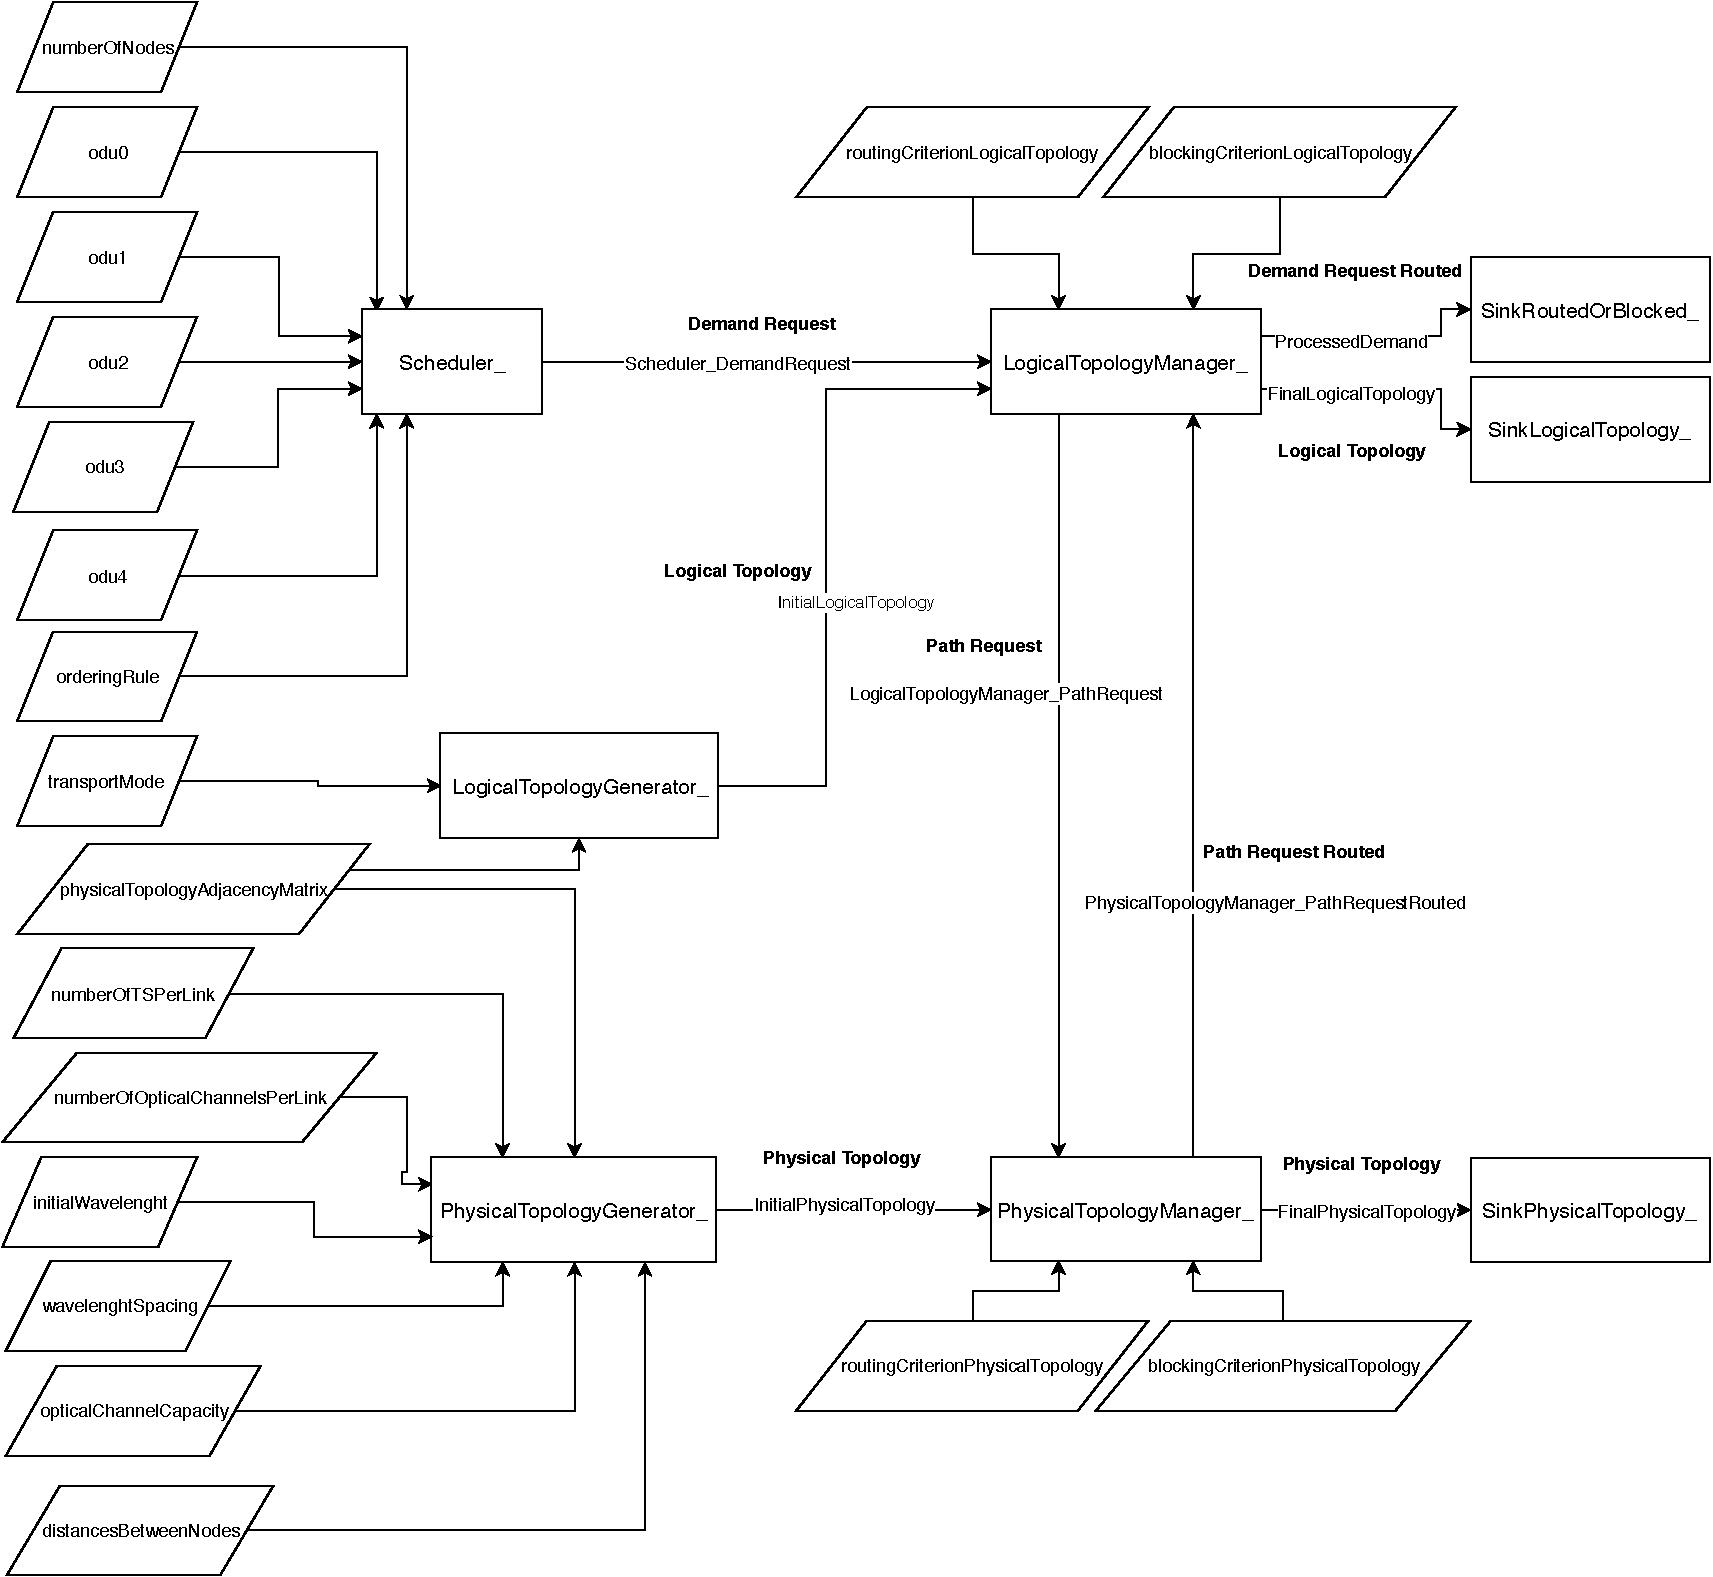
\includegraphics[width=1 \textwidth]{fig/logos/fluxogramaFinalFinal.pdf}
    \caption{Final scheme of the implemented platform.}
    \label{finalPlatformScheme}
  \end{center}
\end{figure}

\section{Chapter summary}

The framework described in the previous chapter \ref{chapter3} was implemented over the NetXPTO-Netplanner simulator. In this chapter is intended to provide a general guideline to simplify its generic use for other users. Starting by a simple explanation of the simulator entry parameters, their meaning and the format in which they are accepted by the system. The various data structures that comprise the different existent signal types are approached and finally is addressed the final report generated by the simulator in the end of each simulation, on which the heuristic results presented in chapter \ref{chapter6} are based.

\cleardoublepage